\documentclass[a4paper, 20pt]{article}
\usepackage[utf8]{inputenc}
\usepackage{paralist}
\usepackage{jeffe,handout}
\usepackage{eqarrays}
\usepackage{tikz}
\usetikzlibrary{matrix}
\usetikzlibrary{arrows,shapes.gates.logic.US,shapes.gates.logic.IEC,calc}
\usepackage{hyperref}
\usepackage{aurical}
\usepackage[T1]{fontenc}

\def\lnot{\mathop{\sim}}
\def\implies{\mathop{\rightarrow}}
\def\xor{\mathop{\oplus}}
\def\iff{\mathop{\leftrightarrow}}

\begin{document}
\headers{CPSC 121}{ }{2019S}

\begin{center}
    \LARGE
    \textbf{HW 1}
    \\[1ex]
    \Large Due: Wednesday, May 15, 2019 at 23:00 \\
\end{center}
    \LARGE
\begin{tabular}{rl}
 & \\
CSID 1: & d6a2b\\
 & \\
CSID 2: & b9i2b\\
 & \\
\end{tabular}
\large

\textbf{Instructions:}
\begin{enumerate}
\item Do not change the problem statements we are giving you. Simply add your solutions by editing this latex document. 
\item If you need more space, add a page between the existing pages using the \texttt{\textbackslash newpage} command.
\item Where possible, include formatting to clearly distinguish your solutions from the given problem text (e.g. use a different font colour for your solutions).
\item Export the completed assignment as a PDF file for upload to gradescope.
\item On Gradescope, upload only \textbf{one} copy per partnership. (Instructions for uploading to Gradescope are posted on the assignments page of the course website.)
\item Late submissions will be accepted up to 24 hours past the deadline with a penalty of 20\% of the assignment's maximum value.
\end{enumerate}

\textbf{Academic Conduct:} 
I certify that my assignment follows the academic conduct rules for of CPSC 121 as outlined on the course website. As part of those rules, when collaborating with anyone outside my group, (1) I and my collaborators took no record but names away, and (2) after a suitable break, my group created the assignment I am submitting without help from anyone other than the course staff. \\

\textbf{Version history:}
\begin{itemize}
    \item 2019-05-08 16:15 -- parenthesis added in Q1a; Q3 gate limit relaxed slightly
    \item 2019-05-05 20:31 -- Initial version for release
\end{itemize}

\newpage
\begin{question}{1.}
\def\StartsWith#1#2{\textit{Starts}({#1},{#2})}

\item[9] Consider the following sets and predicates: 
  \begin{itemize}
  \item $D$: video game developers
  \item $G$: video game titles
  \item $P$: hardware platforms
  \item $M(d, g)$: developer $d$ made game $g$.
  \item $R(g, p)$: game $g$ released on platform $p$.
  \item $B(d, g)$: developer $d$ bribed a journalist to write a favourable review for game $g$.
  \end{itemize}

  Rewrite each of  the following statements using \textbf{only}  the quantifiers $\forall$
  and $\exists$, the predicates $M$, $R$ and $B$, the domains $D$, $G$, $P$, and $\mathbb{R}$ (the set of real numbers),
  logical connectives, and the operators $=$, $\neq$. $<$, $\le$, $\ge$ and $>$.
  
  If you feel a  sentence is ambiguous, then state your assumed interpretation.
  \begin{question}{a.}[2]

  \item[3] Every developer made a game that released on every platform.
   
   \vspace{2.0in}
   
  \item[3] Some developer bribed a journalist to write a favourable review for a game made by a different developer.
  
  \vspace{2.0in}
   
  \item[3] Some developer bribed journalists to write favourable reviews for every game that the developer made.
  
  \vspace{2.0in}

  \end{question}

\newpage
\\1(a).
\\ Proof:
\\ $\equiv \lnot p \land q \land (\lnot s \lor (\lnot r \land s)) \lor (q \land(p \lor (\lnot p \land r \land s)))$ [Start]
\\ $\equiv \lnot p \land q \land (\lnot s \lor (\lnot r \land s)) \lor (q \land((p \lor \lnot p) \land(p \lor r) \land(p \lor s)))$ [DIST]
\\ $\equiv (\lnot p \land q \land ((\lnot s \lor \lnot r) \land (\lnot s \lor s))) \lor (q \land((p \lor \lnot p) \land(p \lor r) \land(p \lor s)))$ [DIST]
\\ $\equiv (\lnot p \land q \land ((\lnot s \lor \lnot r) \land T)) \lor (q \land((p \lor \lnot p) \land(p \lor r) \land(p \lor s)))$ [NEG]
\\ $\equiv (\lnot p \land q \land ((\lnot s \lor \lnot r) \land T)) \lor (q \land(T \land(p \lor r) \land(p \lor s)))$ [NEG]
\\ $\equiv (\lnot p \land q \land (\lnot s \lor \lnot r)) \lor (q \land(T \land(p \lor r) \land(p \lor s)))$ [I]
\\ $\equiv (\lnot p \land q \land (\lnot s \lor \lnot r)) \lor (q \land(p \lor r) \land(p \lor s))$ [I]
\\ $\equiv (q \land \lnot p \land (\lnot s \lor \lnot r)) \lor (q \land(p \lor r) \land(p \lor s))$ [COM]
\\ $\equiv q \land ((\lnot p \land (\lnot s \lor \lnot r)) \lor ((p \lor r) \land(p \lor s)))$ [DIST]
\\ $\equiv q \land ((\lnot p \land (\lnot s \lor \lnot r)) \lor (p \lor (r \land s)))$ [DIST]
\\ $\equiv q \land ((\lnot p \land \lnot (s \land r)) \lor (p \lor (r \land s)))$ [DM]
\\ $\equiv q \land (\lnot (p \lor (s \land r)) \lor (p \lor (r \land s)))$ [DM]
\\ $\equiv q \land (\lnot (p \lor (r \land s)) \lor (p \lor (r \land s)))$ [COM]
\\ $\equiv q \land T$ [NEG]
\\ $\equiv q$ [I]
\\ \boxed{}
\\
\\
\\1(b).
\\ Proof:
\\ $\equiv ((w \land x)\lor(\lnot w \land \lnot x))\land((\lnot y \land \lnot z)\lor(y \land z))\lor \lnot(w \land y)$ [Start]
\\ $\equiv (((w \land x)\lor(\lnot w \land \lnot x))\land((\lnot y \land \lnot z)\lor(y \land z)))\lor \lnot w \lor \lnot y$ [DM]
\\ $\equiv (((w \land x)\lor(\lnot w \land \lnot x))\lor \lnot w \land((\lnot y \land \lnot z)\lor(y \land z))\lor \lnot w ) \lor \lnot y$ [DIST]
\\ $\equiv (((w \land x)\lor(\lnot w \land \lnot x)\lor \lnot w) \land((\lnot y \land \lnot z)\lor(y \land z))\lor \lnot w ) \lor \lnot y$ [ASS]
\\ $\equiv (((w \land x)\lor \lnot w \lor (\lnot w \land \lnot x)) \land((\lnot y \land \lnot z)\lor(y \land z))\lor \lnot w ) \lor \lnot y$ [COM]
\\ $\equiv ((((w \lor \lnot w) \land (x \lor \lnot w)) \lor (\lnot w \land \lnot x)) \land((\lnot y \land \lnot z)\lor(y \land z))\lor \lnot w ) \lor \lnot y$ [DIST]
\\ $\equiv (((T \land (x \lor \lnot w)) \lor (\lnot w \land \lnot x)) \land((\lnot y \land \lnot z)\lor(y \land z))\lor \lnot w ) \lor \lnot y$ [NEG]
\\ $\equiv ((((x \lor \lnot w)) \lor (\lnot w \land \lnot x)) \land((\lnot y \land \lnot z)\lor(y \land z))\lor \lnot w ) \lor \lnot y$ [I]
\\ $\equiv ((((\lnot w \lor x)) \lor (\lnot w \land \lnot x)) \land((\lnot y \land \lnot z)\lor(y \land z))\lor \lnot w ) \lor \lnot y$ [COM]
\\ $\equiv ((\lnot w \lor x \lor (\lnot w \land \lnot x)) \land((\lnot y \land \lnot z)\lor(y \land z))\lor \lnot w ) \lor \lnot y$ [ASS]
\\ $\equiv ((\lnot w \lor (x \lor \lnot w \land x \lor \lnot x)) \land((\lnot y \land \lnot z)\lor(y \land z))\lor \lnot w ) \lor \lnot y$ [DIST]
\\ $\equiv ((\lnot w \lor (x \lor \lnot w \land T)) \land((\lnot y \land \lnot z)\lor(y \land z))\lor \lnot w ) \lor \lnot y$ [NEG]
\\ $\equiv ((\lnot w \lor (x \lor \lnot w)) \land((\lnot y \land \lnot z)\lor(y \land z))\lor \lnot w ) \lor \lnot y$ [I]
\\ $\equiv ((\lnot w \lor x \lor \lnot w) \land((\lnot y \land \lnot z)\lor(y \land z))\lor \lnot w ) \lor \lnot y$ [ASS]
\\ $\equiv ((\lnot w \lor \lnot w \lor x ) \land((\lnot y \land \lnot z)\lor(y \land z))\lor \lnot w ) \lor \lnot y$ [COM]
\\ $\equiv ((\lnot w \lor x ) \land((\lnot y \land \lnot z)\lor(y \land z))\lor \lnot w ) \lor \lnot y$ [ID]
\\ $\equiv ((\lnot w \lor x ) \land \lnot w \lor((\lnot y \land \lnot z)\lor(y \land z)) ) \lor \lnot y$ [COM]
\\ $\equiv \lnot w \lor( x \land((\lnot y \land \lnot z)\lor(y \land z)) ) \lor \lnot y$ [DIST]
\\ $\equiv \lnot w \lor(x \lor \lnot y \land((\lnot y \land \lnot z)\lor(y \land z)) \lor \lnot y ) $ [DIST]
\\ $\equiv \lnot w \lor((x \lor \lnot y) \land((\lnot y \land \lnot z)\lor(y \land z)) \lor \lnot y ) $ [ASS]
\\ $\equiv \lnot w \lor((x \lor \lnot y) \land((\lnot y \land \lnot z)\lor(y \land z) \lor \lnot y )) $ [ASS]
\\ $\equiv \lnot w \lor((x \lor \lnot y) \land((\lnot y \land \lnot z)\lor((y \lor \lnot y) \land (z \lor \lnot y )))) $ [DIST]
\\ $\equiv \lnot w \lor((x \lor \lnot y) \land((\lnot y \land \lnot z)\lor(T \land (z \lor \lnot y )))) $ [NEG]
\\ $\equiv \lnot w \lor((x \lor \lnot y) \land((\lnot y \land \lnot z)\lor((z \lor \lnot y )))) $ [I]
\\ $\equiv \lnot w \lor((x \lor \lnot y) \land((\lnot y \land \lnot z)\lor z \lor \lnot y )) $ [ASS]
\\ $\equiv \lnot w \lor((x \lor \lnot y) \land((\lnot y \lor z) \land (\lnot z \lor z) \lor \lnot y )) $ [ASS]
\\ $\equiv \lnot w \lor((x \lor \lnot y) \land((\lnot y \lor z) \land (\lnot z \lor z) \lor \lnot y )) $ [DIST]
\\ $\equiv \lnot w \lor((x \lor \lnot y) \land((\lnot y \lor z) \land T \lor \lnot y )) $ [NEG]
\\ $\equiv \lnot w \lor((x \lor \lnot y) \land((\lnot y \lor z)  \lor \lnot y )) $ [I]
\\ $\equiv \lnot w \lor((x \lor \lnot y) \land(\lnot y \lor z  \lor \lnot y )) $ [ASS]
\\ $\equiv \lnot w \lor((x \lor \lnot y) \land( z \lor \lnot y \lor \lnot y )) $ [COM]
\\ $\equiv \lnot w \lor((x \lor \lnot y) \land( z \lor \lnot y )) $ [COM]
\\ $\equiv \lnot w \lor(x  \land z)\lor \lnot y $ [DIST]
\\ \boxed{}
\newpage
\item[10] Later in the semester we will discover strategies for proving that for integers $a$, $b$, $c$, $d$, and $m$, if $a\equiv b\bmod{m}$ and $c\equiv d\bmod{m}$, then $a\cdot c\equiv b\cdot d\bmod{m}$, and $a+c\equiv b+d\bmod{m}$. In this problem, we will  investigate the meaning of these statements, and see their implications for number representation. Feel free to use a calculator for parts (a), (b), (f), (g), (h), (i) and (l).

\begin{question}{a.}[0.5]
    \item[0.5] Write the 16-bit unsigned representations of 30924.
    \begin{Questions}
    \vfill
    \end{Questions}
    \item[0.5] What is $30924\bmod 32$, expressed in decimal?
    \begin{Questions}
    \vfill
    \end{Questions}
    \item[0.5] Write the 5-bit unsigned representation of your answer to part (b).
    \begin{Questions}
    \vfill
    \end{Questions}
    \item[0.5] Describe the relationship between your answers to parts (a) and (c).
    \begin{Questions}
    \vfill
    \end{Questions}
    \item[1] Explain how you can compute the remainder when 30924 is divided by 16 (in decimal) \emph{in 10 seconds or less}.
    \begin{Questions}
    \vfill\vfill\eject
    \end{Questions}
    \item[0.5] If $a = 30924$, and $b= 48701$, find the least significant 5 bits of $a+b$ (in binary).
    \begin{Questions}
    \vfill
    \end{Questions}
    \item[0.5] Find $30924 \cdot 8\bmod{32}$ (in decimal).
    \begin{Questions}
    \vfill
    \end{Questions}
    \item[1]
    Write the 16-bit two's complement {\em signed} representation of $-30924$.
    \begin{Questions}
    \vfill
    \end{Questions}
    \item[1]
    Find $-30924\mod{32}$ (in binary).
    \begin{Questions}
    \vfill
    \end{Questions}
    \item[1]
    Describe the relationship between your answers to parts (c) and (i).
    \begin{Questions}
    \vfill\vfill
    \end{Questions}
    \item[0.5] If $a = -30924$, and $b= 16653$, find the least significant 5 bits of $a+b$ (in binary).
    \begin{Questions}
    \vfill
    \end{Questions}
    \item[0.5] Find $-30924 \cdot 8\mod{32}$ (in decimal).
    \begin{Questions}
    \vfill\eject
    \end{Questions}
    \item[2]
    By exploration, we have illustrated some of the implications of the simple rules of modular arithmetic. Show that the rule cannot be extended to the division operation, by finding a {\em counter example}. That is, find unsigned integers $a$, $b$, $c$, $d$, and $m$, so that $a\equiv b\mod{m}$ and $c\equiv d\mod{m}$, but $a/c\not\equiv b/d\mod{m}$.
    \begin{Questions}
    \vfill
    \end{Questions}
    
\end{question}
\vfill\eject

\\2(a). B \equiv D
\\ expression 1, expression 2, reason
\\$(\lnot a \lor b)\land(\lnot a \lor c)\land(\lnot a \lor \lnot d) \equiv a \implies (b \land c \land \lnot d)$ [Start]
\\$(\lnot a \lor b)\land(\lnot a \lor c)\land(\lnot a \lor \lnot d) \equiv \lnot a \lor (b \land c \land \lnot d)$ [IMP]
\\$\lnot a \lor (b \land c \land \lnot d) \equiv \lnot a \lor (b \land c \land \lnot d)$ [DIST]
\\
\\2(b). A \equiv E
\\ expression 1, expression 2, reason
\\$ (\lnot a \land b) \iff \lnot(c \lor d) \equiv \lnot ((a \lor \lnot b \lor c \lor d) \land ((\lnot a \land b) \lor \lnot (c \lor d)))$ [Start]
\\$ \lnot ((\lnot a \land b) (+) \lnot(c \lor d)) \equiv \lnot ((a \lor \lnot b \lor c \lor d) \land ((\lnot a \land b) \lor \lnot (c \lor d)))$ [Equivalence definition]
\\$  \lnot (\lnot ((\lnot a \land b) \land \lnot (c \lor d)) \land ((\lnot a \land b) \lor \lnot (c \lor d))) \equiv \lnot ((a \lor \lnot b \lor c \lor d) \land ((\lnot a \land b) \lor \lnot (c \lor d)))$ [Xor definition]
\\$  \lnot (\lnot ((\lnot a \land b) \land \lnot (c \lor d)) \land ((\lnot a \land b) \lor \lnot (c \lor d))) \equiv \lnot ((\lnot( \lnot a \land b) \lor c \lor d) \land ((\lnot a \land b) \lor \lnot (c \lor d)))$ [DM]
\\$  \lnot (\lnot ((\lnot a \land b) \land \lnot (c \lor d)) \land ((\lnot a \land b) \lor \lnot (c \lor d))) \equiv \lnot ((\lnot( \lnot a \land b) \lor (c \lor d)) \land ((\lnot a \land b) \lor \lnot (c \lor d)))$ [ASS]
\\$  \lnot (\lnot ((\lnot a \land b) \land \lnot (c \lor d)) \land ((\lnot a \land b) \lor \lnot (c \lor d))) \equiv \lnot (\lnot(( \lnot a \land b) \land \lnot (c \lor d)) \land ((\lnot a \land b) \lor \lnot (c \lor d)))$ [DM]
\\
\\3(c). C $\equiv$ F
\\ Truth table of C:
\\
\begin{displaymath}
\begin{array}{|c c c c|c|c|c|}
a & b & c & d & (a \land b \land c)&\lnot(b \land c \land d)&f \equiv (a \land b \land c)\lor \lnot(b \land c \land d)\\
\hline 
1&1&1&X&1&X&1\\
X&0&X&X&X&1&1\\
X&X&0&X&X&1&1\\
X&X&X&0&X&1&1\\
\end{array}
\end{displaymath}
\\ Since the statement is separated by an Or gate, we can find what makes either terms true and ignore the other term. That lets us deduce the truth table quickly. Unmentioned input combination(s) is false.
\\
\\ Truth table of F:
\\
\begin{displaymath}
\begin{array}{|c c c c|c|c|c|c|c|}
a & b & c & d & w \equiv (c (+) d) & x \equiv \lnot (a (+) b) & y \equiv \lnot (c \lor d) & z \equiv (a \land \lnot b) & f = w \lor x \lor y \lor z\\
\hline 
0 & 0 & 0 & 0 &0&1&1&0&1\\
0 & 0 & 0 & 1 &1&1&0&0&1\\
0 & 0 & 1 & 0 &1&1&0&0&1\\
0 & 0 & 1 & 1 &0&1&0&0&1\\
0 & 1 & 0 & 0 &0&0&1&0&1\\
0 & 1 & 0 & 1 &1&0&0&0&1\\
0 & 1 & 1 & 0 &1&0&0&0&1\\
0 & 1 & 1 & 1 &0&0&0&0&0\\
1 & 0 & 0 & 0 &0&0&1&1&1\\
1 & 0 & 0 & 1 &1&0&0&1&1\\
1 & 0 & 1 & 0 &1&0&0&1&1\\
1 & 0 & 1 & 1 &0&0&0&1&1\\
1 & 1 & 0 & 0 &0&1&1&0&1\\
1 & 1 & 0 & 1 &1&1&0&0&1\\
1 & 1 & 1 & 0 &1&1&0&0&1\\
1 & 1 & 1 & 1 &0&1&0&0&1\\
\end{array}
\end{displaymath}
\\
\\ These two truth tables' output values are the same for given input value (ie only 0111 input makes output 0), therefore the two logical statements are equivalent.
\newpage
\item[17] Logical Arguments
\begin{question}{a.}[5]

\item[4] Consider the following argument:
\begin{quote}
If there is a chance of rain, or he ate bean chili for lunch, Geoff will not ride his bicycle. Unless Geoff washed his car in the morning, there is no chance of rain. Today Geoff neither washed his car nor ate bean chili. Therefore, Geoff will ride his bicycle today.
\end{quote}

First represent this argument symbolically. Then determine whether it is valid or not.
Justify your answer.
\begin{Questions}
\vfill\eject
\end{Questions}

\item[4] Consider the following argument:
\begin{quote}
If Geoff works hard enough and does not get fired, then he will get paid. If he gets paid, then he will buy food to eat. Geoff has not bought food to eat. Therefore either Geoff did not work hard enough, or he got fired.
\end{quote}

First represent this argument symbolically. Then determine whether it is valid or not.
Justify your answer.
\begin{Questions}
\vfill\eject
\end{Questions}

\item [5]
Consider the following argument:
\begin{quote}
If 30,000 cookies disappeared from Christie's factory, then either Christie destroyed the cookies, or Keebler stole the cookies. If it is not the case that a tree-dwelling elf became the new CEO of Christie and the new Christie CEO colluded with Keebler, then 30,000 cookies disappeared from Christie's factory. If the new Christie CEO did not have a secret meeting with Keebler's industrial spies, then Keebler did not steal the cookies. Christie did not destroy the cookies, and the new Christie CEO had a secret meeting with Keebler's spies. Therefore, Christie's new CEO did not collude with Keebler! No collusion!
\end{quote}

First represent this argument symbolically. Then determine whether it is valid or not.
Justify your answer.
\begin{Questions}
\vfill\eject
\end{Questions}

\item[4]
Determine whether the following argument is valid. If it is valid, show a formal proof and if it is invalid provide a counter-example, i.e. an assignment of truth values that demonstrate a contradiction.


This argument is \underline{~~~~~~~~~~~~~~~~~~~~~}. (Fill in the blank with ``valid'' or ``invalid''.)
\vspace{0.2in}

\hspace{0.4in}\begin{tabular}{r}

$\lnot p \land q$\\
$r \rightarrow p$\\
$\lnot r \rightarrow (s \land t)$\\
$s \rightarrow (t \lor p)$\\
\hline
$\therefore  t  $\\
\end{tabular}
\vspace{0.2in}

Proof:

\hspace{0.4in}\begin{tabular}{r|l}
~~~~~~inference~~~~~~ & rule \\
\hline
 & ~~~~~~~~~~~~~~~~~~~~~~~\\
\hline
 & ~~~~~~~~~~~~~~~~~~~~~~~\\
\hline
 & ~~~~~~~~~~~~~~~~~~~~~~~\\
\hline
 & ~~~~~~~~~~~~~~~~~~~~~~~\\
\hline
 & ~~~~~~~~~~~~~~~~~~~~~~~\\
\hline
 & ~~~~~~~~~~~~~~~~~~~~~~~\\
\hline
 & ~~~~~~~~~~~~~~~~~~~~~~~\\
\hline
 & ~~~~~~~~~~~~~~~~~~~~~~~\\
\hline
 & ~~~~~~~~~~~~~~~~~~~~~~~\\
\hline
 & ~~~~~~~~~~~~~~~~~~~~~~~\\
\hline
 & ~~~~~~~~~~~~~~~~~~~~~~~\\
\hline
 & ~~~~~~~~~~~~~~~~~~~~~~~\\
\hline
 & ~~~~~~~~~~~~~~~~~~~~~~~\\
\hline
 & ~~~~~~~~~~~~~~~~~~~~~~~\\
\hline
 & ~~~~~~~~~~~~~~~~~~~~~~~\\
\hline
\end{tabular}
\large
\vspace{0.2in}

Invalidating truth assignment:\bigskip

$r=~~~~~~$, $s=~~~~~~$, $t=~~~~~~$, $u=~~~~~~$, $w=~~~~~~$


\end{question}
\newpage

\newpage
\\3(a).
\\
\leavevmode\lower45pt\hbox{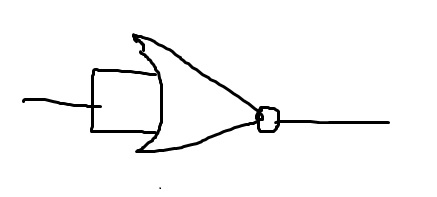
\includegraphics[scale=0.75]{3a.jpg}}
\\Proof:
\\ $ \equiv \lnot (a \lor a)$ [Start]
\\ $ \equiv \lnot (a)$ [ID]
\\ $ \equiv \lnot a$ [ASS]
\\ \boxed{}
\\
\\3(b).
\\
\leavevmode\lower45pt\hbox{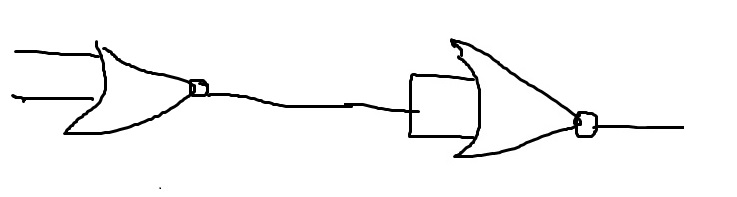
\includegraphics[scale=0.75]{3b.jpg}}
\\ Proof:
\\ $ \equiv \lnot (\lnot (a \lor b) \lor \lnot (a \lor b))$ [Start]
\\ $ \equiv \lnot (\lnot (a \lor b))$ [ID]
\\ $ \equiv (a \lor b)$ [DNEG]
\\ \boxed{}
\\
\\3(c).
\\
\leavevmode\lower45pt\hbox{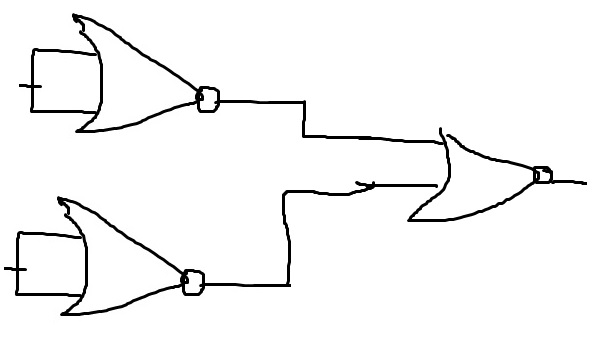
\includegraphics[scale=0.75]{3c.jpg}}
\begin{displaymath}
\begin{array}{|c c|c|c|c|c|}
a & b & \lnot (a \lor a) \equiv \lnot a & \lnot (b \lor b) \equiv \lnot b & \lnot (\lnot (a \lor a) \lor \lnot (b \lor b)) \equiv \lnot (\lnot a \lor \lnot b) & a \land b\\
\hline 
0 & 0 & 1 & 1 & 0 & 0\\
0 & 1 & 1 & 0 & 0 & 0\\
1 & 0 & 0 & 1 & 0 & 0\\
1 & 1 & 0 & 0 & 1 & 1\\
\end{array}
\end{displaymath}
\\3(d).
\\ Since the question didn't specify how we should simplify the truth table, I will use K-map for simplicity:
\begin{displaymath}
\begin{array}{|c|c|c|c|c|}
- & x1 \land x0 & \lnot x1 \land x0 & \lnot x1 \land \lnot x0 & x1 \land \lnot x0 \\
\hline 
x3 \land x2 & 0&1&1&0\\
\lnot x3 \land x2 & 0&0&1&0\\
\lnot x3 \land \lnot x2 & 0&0&0&1\\
x3 \land \lnot x2 & 0&0&0&1\\
\end{array}
\end{displaymath}
\\ Finding sum of minterms, I can get:
\\ $f \equiv (x2 \land \lnot x1 \land \lnot x0) \lor (x3 \land x2 \land \lnot x1) \lor (\lnot x2 \land x1 \land \lnot x0)$
\\
\\ I can use logical properties to change the logical statement into one that's made up of only Nor gates:
\\
\\ Proof:
\\ $\equiv (x2 \land \lnot x1 \land \lnot x0) \lor (x3 \land x2 \land \lnot x1) \lor (\lnot x2 \land x1 \land \lnot x0)$ [Start]
\\ $\equiv \lnot (\lnot x2 \lor x1 \lor x0) \lor \lnot (\lnot x3 \lor \lnot x2 \lor x1) \lor \lnot (x2 \lor \lnot x1 \lor x0)$ [DM to all And terms]
\\ $\equiv \lnot (\lnot (x2 \lor x2) \lor x1 \lor x0) \lor \lnot (\lnot (x3 \lor x3) \lor \lnot (x2 \lor x2) \lor x1) \lor \lnot (x2 \lor \lnot (x1 \lor x1) \lor x0)$ [ID to all Not terms]
\\ $\equiv \lnot (\lnot (\lnot (\lnot (x2 \lor x2) \lor x1 \lor x0) \lor \lnot (\lnot (x3 \lor x3) \lor \lnot (x2 \lor x2) \lor x1) \lor \lnot (x2 \lor \lnot (x1 \lor x1) \lor x0)))$ [DNEG]
\\ \boxed{}
\\
\\ This logical statement can be simplified further, but it already uses under 16 gates, as shown here:
\\ 
\leavevmode\lower45pt\hbox{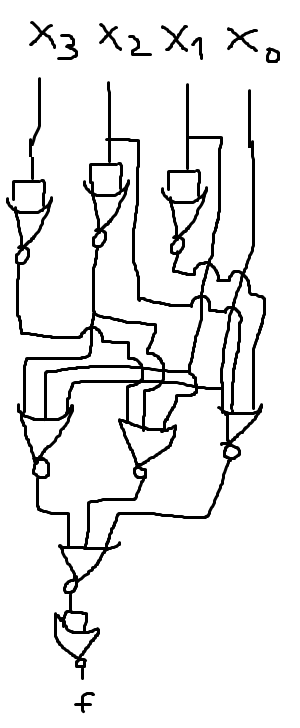
\includegraphics[scale=0.75]{3d.jpg}}
\newpage
 \item[8] Using mathematical induction, prove that
 \begin{displaymath}
 \sum_{i=1}^n (i-1) 2^i = (n-2)2^{n+1}
 + 4
 \end{displaymath}
 
 \begin{Questions}
 \\{\color{NavyBlue}
 \\Proof:
 \\
 \\Part 1: Base case
 \begin{gather}
 (n-1) 2^n = (n-2)2^{n+1}+ 4
 \\(1-1) 2^1 = (1-2)2^{1+1}+ 4
 \\0 = 0
 \end{gather}
 \\Part 2: Induction step
 \\
 \\ Assuming that n case is true, we have to prove that this statement is true: 
 \begin{gather}
 \sum_{i=1}^{n+1} (i-1) 2^i = ((n+1)-2)2^{(n+1)+1}+ 4
 \end{gather}
 \\To prove that [4] is true, we say that the sum of n+1 terms is equals to the sum of n terms plus the n+1th term, and simplify from there:
  \begin{gather}
 \sum_{i=1}^{n+1} (i-1) 2^i = \sum_{i=1}^n (i-1) 2^i + ((n+1)-1) 2^{n+1}
 \\ ((n+1)-2)2^{(n+1)+1}+ 4 = ((n-2)2^{n+1}
 + 4) + ((n+1)-1) 2^{n+1}
 \\ (n-1)2^{n+2}+ 4 = (n-2)2^{n+1}
  + n 2^{n+1} + 4
  \\ (n-1)2^{n+2}= (n-2)2^{n+1}
  + n 2^{n+1}
   \\ n2^{n+2} - 2^{n+2} = (n-2)2^{n+1}
  + n 2^{n+1}
   \\ n2^{n+2} - 2^{n+2} = n2^{n+1} - 2^{n+2}
  + n 2^{n+1}
    \\ n2^{n+2} - 2^{n+2} = n2^{n+1} - 2^{n+2}
  + n 2^{n+1}
     \\ n2^{n+2} - 2^{n+2} = 2n2^{n+1} - 2^{n+2}
     \\ n2^{n+2} - 2^{n+2} = n2^{n+2} - 2^{n+2}
 \end{gather}
 \\Steps 5-7 is substituting terms. Step 8 cancels 4 from both sides. Steps 9-10 expands (n-1) and (n-2) terms by distributive property. Steps 11-13 combine like terms to get the final equality. 
 \\Thus, we have proved that when n case is true, n+1 case is true as well. 
 \\}
 \begin{figure}
\begin{verbatim}
         _______                   _____                    _____          
        /::\    \                 /\    \                  /\    \         
       /::::\    \               /::\    \                /::\    \        
      /::::::\    \             /::::\    \              /::::\    \       
     /::::::::\    \           /::::::\    \            /::::::\    \      
    /:::/~~\:::\    \         /:::/\:::\    \          /:::/\:::\    \     
   /:::/    \:::\    \       /:::/__\:::\    \        /:::/  \:::\    \    
  /:::/    / \:::\    \     /::::\   \:::\    \      /:::/    \:::\    \   
 /:::/____/   \:::\____\   /::::::\   \:::\    \    /:::/    / \:::\    \  
|:::|    |     |:::|    | /:::/\:::\   \:::\    \  /:::/    /   \:::\ ___\ 
|:::|____|     |:::|____|/:::/__\:::\   \:::\____\/:::/____/     \:::|    |
 \:::\   _\___/:::/    / \:::\   \:::\   \::/    /\:::\    \     /:::|____|
  \:::\ |::| /:::/    /   \:::\   \:::\   \/____/  \:::\    \   /:::/    / 
   \:::\|::|/:::/    /     \:::\   \:::\    \       \:::\    \ /:::/    /  
    \::::::::::/    /       \:::\   \:::\____\       \:::\    /:::/    /   
     \::::::::/    /         \:::\   \::/    /        \:::\  /:::/    /    
      \::::::/    /           \:::\   \/____/          \:::\/:::/    /     
       \::::/____/             \:::\    \               \::::::/    /      
        |::|    |               \:::\____\               \::::/    /       
        |::|____|                \::/    /                \::/____/        
         ~~                       \/____/                  ~~                  
\end{verbatim}
\caption{A blessed QED to end a blessed proof}
\end{figure}

 \vfill\eject
 \clearpage
 \end{Questions}
 
\newpage
\\ 4.
\\ I know that in the range of [0, 31] the prime numbers are:  2, 3, 5, 7, 11, 13, 17, 19, 23, 29, 31. I can write a truth table from these outputs. 
\begin{displaymath}
\begin{array}{|c c c c c|c|c|}
x4&x3&x2&x1&x0&Decimal&z\\
\hline 
0 & 0 & 0 & 0 & 0 & 0&0\\
0 & 0 & 0 & 0 & 1 & 1&0\\
0 & 0 & 0 & 1 & 0 & 2&1\\
0 & 0 & 0 & 1 & 1 &3&1\\
0 & 0 & 1 & 0 & 0 &4&0\\
0 & 0 & 1 & 0 & 1 &5&1\\
0 & 0 & 1 & 1 & 0 &6&0\\
0 & 0 & 1 & 1 & 1 &7&1\\
0 & 1 & 0 & 0 & 0 &8&0\\
0 & 1 & 0 & 0 & 1 &9&0\\
0 & 1 & 0 & 1 & 0 &10&0\\
0 & 1 & 0 & 1 & 1 &11&1\\
0 & 1 & 1 & 0 & 0 &12&0\\
0 & 1 & 1 & 0 & 1 &13&1\\
0 & 1 & 1 & 1 & 0 &14&0\\
0 & 1 & 1 & 1 & 1 &15&0\\
1 & 0 & 0 & 0 & 0 &16&0\\
1 & 0 & 0 & 0 & 1 &17&1\\
1 & 0 & 0 & 1 & 0 &18&0\\
1 & 0 & 0 & 1 & 1 &19&1\\
1 & 0 & 1 & 0 & 0 &20&0\\
1 & 0 & 1 & 0 & 1 &21&0\\
1 & 0 & 1 & 1 & 0 &22&0\\
1 & 0 & 1 & 1 & 1 &23&1\\
1 & 1 & 0 & 0 & 0 &24&0\\
1 & 1 & 0 & 0 & 1 &25&0\\
1 & 1 & 0 & 1 & 0 &26&0\\
1 & 1 & 0 & 1 & 1 &27&0\\
1 & 1 & 1 & 0 & 0 &28&0\\
1 & 1 & 1 & 0 & 1 &29&1\\
1 & 1 & 1 & 1 & 0 &30&0\\
1 & 1 & 1 & 1 & 1 &31&1\\
\end{array}
\end{displaymath}
\\ Since the question did not specify the method, I can use K-map made from this truth table to get logical statement of $z$:
\\
\begin{displaymath}
\begin{array}{|c|c|c|c|c|}
- & x1 \land x0 & \lnot x1 \land x0 & \lnot x1 \land \lnot x0 & x1 \land \lnot x0 \\
\hline 
x4 \land x3 \land x2 & 1&1&0&0\\
x4 \land \lnot x3 \land x2 & 1&0&0&0\\
x4 \land \lnot x3 \land \lnot x2 & 1&1&0&0\\
x4 \land x3 \land \lnot x2 & 0&0&0&0\\
\lnot x4 \land x3 \land \lnot x2 & 1&0&0&0\\
\lnot x4 \land \lnot x3 \land \lnot x2 & 1&0&0&1\\
\lnot x4 \land \lnot x3 \land x2 & 1&1&0&0\\
\lnot x4 \land x3 \land x2 & 0&1&0&0\\
\end{array}
\end{displaymath}
\\
\\ We can rewrite these two K-maps into logical statements as follow:
\\ $ z = (x3 \land x2 \land \lnot x1 \land x0) \lor (\lnot x4 \land \lnot x3 \land x2 \land x0) \lor (\lnot x4 \land \lnot x3 \land \lnot x2 \land x1) \lor (\lnot x4 \land \lnot x2 \land x1 \land x0) \lor (x4 \land \lnot x3 \land \lnot x2 \land x0) \lor (x4 \land x2 \land x1 \land x0) $
\\
\\ Using K-map, we can be sure that this is the most simplified form of the logical statement. While there are one Xor and one Xnor simplifications we can make with $(4(+)2)$ and $\lnot (4(+)2)$, it doesn't decrease the number of logic gates since we still need to wrap the Xor and Xnor with an And gate (respectively) to pair it with other terms ($(\lnot x3 \land x0)$ and $(x1 \land x0)$, respectively). We can make this into a logic circuit:
\\
\leavevmode\lower45pt\hbox{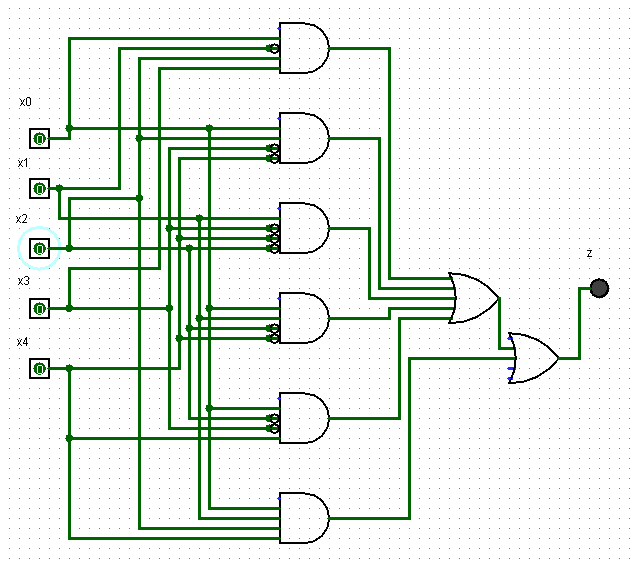
\includegraphics[scale=0.75]{4.PNG}}
\\
\\ Note that I have to use two separate Or gates at the output since Logisim has 5 input maximum for their Or gate.
\\
\\ 
\end{question}
\end{document}